\documentclass[addpoints,spanish, 12pt,a4paper]{exam}
%\documentclass[answers, spanish, 12pt,a4paper]{exam}
\printanswers
\pointpoints{punto}{puntos}
\hpword{Puntos:}
\vpword{Puntos:}
\htword{Total}
\vtword{Total}
\hsword{Resultado:}
\hqword{Ejercicio:}
\vqword{Ejercicio:}

\usepackage[utf8]{inputenc}
\usepackage[spanish]{babel}
\usepackage{eurosym}
%\usepackage[spanish,es-lcroman, es-tabla, es-noshorthands]{babel}


\usepackage[margin=1in]{geometry}
\usepackage{amsmath,amssymb}
\usepackage{multicol}
\usepackage{yhmath}
\usepackage{pdflscape}

\pointsinrightmargin % Para poner las puntuaciones a la derecha. Se puede cambiar. Si se comenta, sale a la izquierda.
\extrawidth{-2.4cm} %Un poquito más de margen por si ponemos textos largos.
\marginpointname{ \emph{\points}}

\usepackage{graphicx}
\graphicspath{{../img/}} 

\newcommand{\class}{1º Bachillerato CCSS}
\newcommand{\examdate}{\today}
\newcommand{\examnum}{Examen final 2ª Evaluación}
\newcommand{\tipo}{A}


\newcommand{\timelimit}{50 minutos}

\renewcommand{\solutiontitle}{\noindent\textbf{Solución:}\enspace}


\pagestyle{head}\firstpageheader{
\includegraphics[width=0.2\columnwidth]{header_left}}{\textbf{Departamento de Matemáticas\linebreak \class}\linebreak \examnum}{
\includegraphics[width=0.1\columnwidth]{header_right}}
\runningheader{\class}{\examnum}{Página \thepage\ of \numpages}
\runningheadrule


\begin{document}

\noindent
\begin{tabular*}{\textwidth}{l @{\extracolsep{\fill}} r @{\extracolsep{6pt}} }
\textbf{Nombre:} \makebox[3.5in]{\hrulefill} & \textbf{Fecha:}\makebox[1in]{\hrulefill} \\
 & \\
\textbf{Tiempo: \timelimit} & Tipo: \tipo 
\end{tabular*}
\rule[2ex]{\textwidth}{2pt}
Esta prueba tiene \numquestions\ ejercicios. La puntuación máxima es de \numpoints. 
La nota final de la prueba será la parte proporcional de la puntuación obtenida sobre la puntuación máxima. 

\begin{center}


\addpoints
 %\gradetable[h][questions]
	\pointtable[h][questions]
\end{center}

\noindent
\rule[2ex]{\textwidth}{2pt}

\begin{questions}

\question[1] Se valorará en este apartado el correcto uso de la notación matemática tanto de la parte de estadística como de probabilidad

\question Las notas en Matemáticas, Física y Lengua respectivamente de 3 alumnos de una clase han sido:
\begin{itemize}
    \item María: 9, 8 ,6
    \item Juan: 7, 7, 3
    \item Luis: 4, 5, 9
\end{itemize}

\begin{parts}
\part[1] Determina el coeficiente de correlación entre las notas de Matemáticas y Física.
\begin{solution}
\\
\begin{tabular}{lrrrrr}
\hline
        &        x &        y &   $x\cdot y$ &    $x^2$ &   $y^2$ \\
\hline
 0      &  9       &  8       &           72 &  81      &      64 \\
 1      &  7       &  7       &           49 &  49      &      49 \\
 2      &  4       &  5       &           20 &  16      &      25 \\
 Sumas  & 20       & 20       &          141 & 146      &     138 \\
 Medias &  6.66667 &  6.66667 &           47 &  48.6667 &      46 \\
\hline
\end{tabular}
\\ \\ Las medias son: \\$\overline{x}=\frac{\Sigma{x_i}}{N}=\frac{20.0}{3}=6.66666666666667$. $\overline{y}=\frac{\Sigma{y_i}}{N}=\frac{20.0}{3}=6.66666666666667$.  El centro de gravedad es: $(6.66666666666667,6.66666666666667)$ \\ \\ Varianzas y covarianzas: \\ $\sigma_x=\sqrt{\frac{\sum{x_i^2}}{N}-\overline{x}^2}=\sqrt{\frac{146.0}{3}-6.66666666666667^2}=2.05480466765632$.\\ $\sigma_y=\sqrt{\frac{\sum{y_i^2}}{N}-\overline{y}^2}=\sqrt{\frac{138.0}{3}-6.66666666666667^2}=1.24721912892464$.\\ $\sigma_{xy}=\frac{\sum{x_i \cdot y_i}}{N}-\overline{x}\cdot \overline{y}=\frac{141.0}{3}-6.66666666666667\cdot 6.66666666666667=2.55555555555555$. \\ \\ Correlación: \\ $r=\dfrac{\sigma_{xy}}{\sigma_x \cdot \sigma_y}=\frac{2.55555555555555}{2.05480466765632\cdot 1.24721912892464}=0.997176464952739$. \\ \\ Recta de regresión: \\ La pendiente es: 0.605263157894737, la ordenada en el origen: 2.63157894736842, El coeficiente de correlación:0.997176464952738 y la recta de regresión: $y = 0.605263157894737 x + 2.63157894736842$
\end{solution}
% \part[1] Determina el coeficiente de correlación entre las notas de Matemáticas y Lengua.
% \begin{solution}
% \\
% \begin{tabular}{lrrrrr}
% \hline
%         &        x &   z &   $x\cdot z$ &    $x^2$ &   $z^2$ \\
% \hline
%  0      &  9       &   6 &           54 &  81      &      36 \\
%  1      &  7       &   3 &           21 &  49      &       9 \\
%  2      &  4       &   9 &           36 &  16      &      81 \\
%  Sumas  & 20       &  18 &          111 & 146      &     126 \\
%  Medias &  6.66667 &   6 &           37 &  48.6667 &      42 \\
% \hline
% \end{tabular}
% \\ \\ Las medias son: \\$\overline{x}=\frac{\Sigma{x_i}}{N}=\frac{20.0}{3}=6.66666666666667$. $\overline{z}=\frac{\Sigma{z_i}}{N}=\frac{18.0}{3}=6.0$.  El centro de gravedad es: $(6.66666666666667,6.0)$ \\ \\ Varianzas y covarianzas: \\ $\sigma_x=\sqrt{\frac{\sum{x_i^2}}{N}-\overline{x}^2}=\sqrt{\frac{146.0}{3}-6.66666666666667^2}=2.05480466765632$.\\ $\sigma_z=\sqrt{\frac{\sum{z_i^2}}{N}-\overline{z}^2}=\sqrt{\frac{126.0}{3}-6.0^2}=2.44948974278318$.\\ $\sigma_{xz}=\frac{\sum{x_i \cdot z_i}}{N}-\overline{x}\cdot \overline{z}=\frac{111.0}{3}-6.66666666666667\cdot 6.0=-3.0$. \\ \\ Correlación: \\ $r=\dfrac{\sigma_{xz}}{\sigma_x \cdot \sigma_z}=\frac{-3.0}{2.05480466765632\cdot 2.44948974278318}=-0.59603956067927$. \\ \\ Recta de regresión: \\ La pendiente es: -0.710526315789474, la ordenada en el origen: 10.7368421052632, El coeficiente de correlación:-0.59603956067927 y la recta de regresión: $y = 10.7368421052632 - 0.710526315789474 x$
% \end{solution}
% \part[1] Interpreta la correlación obtenida.
% \part[2] Ana es una alumna de la clase que ha faltado al examen de Lengua pero sabemos que en Matemáticas tiene un 6. Estima la nota de Lengua a partir de la recta de regresión correspondiente.
% \begin{solution}
% $y = 6.47368421052632$
% \end{solution}
\part[1] Sonia es una alumna de la clase que ha faltado al examen de Física pero sabemos que en Matemáticas tiene un 9. Estima la nota de Física a partir de la recta de regresión correspondiente.
\begin{solution}
$y = 8.07894736842105 $
\end{solution}

% \part[1] Interpreta el resultado anterior indicando cómo de buena es la estimación.
\end{parts}

% \question Sean x = “gastos en publicidad de un producto” (en miles de euros) e y = “ventas conseguidas de
% ese producto” (en miles de euros)\\
% \begin{tabular}{|c||c|c|c|c|c|c|c|c|}
% \hline 
% X & 1 & 2 & 3 & 4 & 5 & 6  \\ 
% \hline 
% y & 10 & 17 & 30 & 28 & 39 & 47 \\ 
% \hline 
% \end{tabular} 
% \begin{parts}
% \part[1] Calcula el coeficiente de correlación.\begin{solution}
% \begin{tabular}{lrrrrr}
% \hline
%         &    x &     y &   $x\cdot y$ &   $x^2$ &    $y^2$ \\
% \hline
%  0      &  1   &  10   &         10   &  1      &  100     \\
%  1      &  2   &  17   &         34   &  4      &  289     \\
%  2      &  3   &  30   &         90   &  9      &  900     \\
%  3      &  4   &  28   &        112   & 16      &  784     \\
%  4      &  5   &  39   &        195   & 25      & 1521     \\
%  5      &  6   &  47   &        282   & 36      & 2209     \\
%  Sumas  & 21   & 171   &        723   & 91      & 5803     \\
%  Medias &  3.5 &  28.5 &        120.5 & 15.1667 &  967.167 \\
% \hline
% \end{tabular}
% \\ \\ Las medias son: \\$\overline{x}=\frac{\Sigma{x_i}}{N}=\frac{21.0}{6}=3.5$. $\overline{y}=\frac{\Sigma{y_i}}{N}=\frac{171.0}{6}=28.5$.  El centro de gravedad es: $(3.5,28.5)$ \\ \\ Varianzas y covarianzas\\ $\sigma_x=\sqrt{\frac{\sum{x_i^2}}{N}-\overline{x}^2}=\sqrt{\frac{91.0}{6}-3.5^2}=1.70782512765993$.\\ $\sigma_y=\sqrt{\frac{\sum{y_i^2}}{N}-\overline{y}^2}=\sqrt{\frac{5803.0}{6}-28.5^2}=12.4465524008324$.\\ $\sigma_{xy}=\frac{\sum{x_i \cdot y_i}}{N}-\overline{x}\cdot \overline{y}=\frac{723.0}{6}-3.5\cdot 28.5=20.75$. \\ \\ Correlación\\ $r=\dfrac{\sigma_{xy}}{\sigma_x \cdot \sigma_y}=\frac{20.75}{1.70782512765993\cdot 12.4465524008324}=0.976170389753606$.
% \end{solution}
% \part[1] Comenta la influencia del gasto publicitario en las ventas.
% \begin{solution}
% La correlación es muy fuerte (se acerca a uno) y positiva. Las ventas aumentan de forma lineal conforme se aumenta el gasto publicitario.
% \end{solution}
% \part[1] Halla la ecuación de la recta de regresión de las ventas respecto del gasto publicitario.\begin{solution}
%  Recta de regresión: \\ La pendiente es: 7.11428571428571, la ordenada en el origen: 3.6, El coeficiente de correlación:0.976170389753606 y la recta de regresión: $y = 7.11428571428571 x + 3.6$
% \end{solution}
% \part[1] Halla las ventas esperadas para un gasto en publicidad de 3200 euros.\begin{solution}
% $y(3.2)=7.11428571428571 \cdot 3.2 + 3.6=26.3657142857143$
% \end{solution}
% \end{parts} 

% \question La temperatura media en los meses de invierno en varias ciudades y el gasto medio por habitante en
% calefacción ha sido:\\
% \begin{tabular}{|c||c|c|c|c|c|c|}
% \hline 
% Temperatura (ºC) & 10 & 12 & 14 & 16  \\ 
% \hline 
% Gasto (\euro ) & 150 & 120 & 102 & 90  \\ 
% \hline 
% \end{tabular} 
% \addpoints % to omit double points count

% \begin{parts}
% \part[1] ¿Cuál es el gasto medio?

% \begin{solution}
% \begin{tabular}{rrrrrr}
% \hline
%     &   x &     y &   xy &   x2 &    y2 \\
% \hline
%   0 &  10 & 150   & 1500 &  100 & 22500 \\
%   1 &  12 & 120   & 1440 &  144 & 14400 \\
%   2 &  14 & 102   & 1428 &  196 & 10404 \\
%   3 &  16 &  90   & 1440 &  256 &  8100 \\
%   \hline
%   4 &  52 & 462   & 5808 &  696 & 55404 \\
%   \hline
%   5 &  13 & 115.5 & 1452 &  174 & 13851 \\
% \hline
% \end{tabular}
% Gasto medio = 115.5
% \end{solution}
% \part[1] Halla el coeficiente de correlación lineal e interprétalo
% \begin{solution}
% covarianza	-49.5 \\
% desvx	2.23606797749979 \\
% desvy	22.599778759979046 \\
% coefcorr -0.9795260923726159 \\
% \end{solution}
% \part[1] Estima el gasto medio por habitante de una ciudad si la temperatura media hubiera sido de 11ºC 

% \begin{solution}
% $y = -9.9x + 244.2$ \\
% 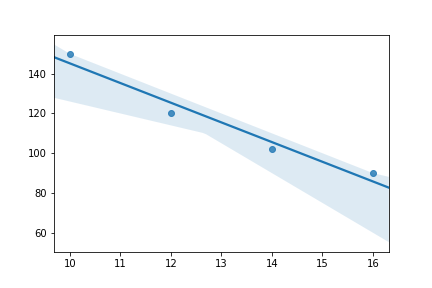
\includegraphics[scale=.5]{regresion1.png} \\
% Valor estimado para 11: 135.3 \euro 
% \end{solution}

% \end{parts}

        \question Se dispone de dos cajas, la caja A contiene 3 bolas moradas y 2 bolas rojas; mientras que la caja B contiene 4
    bolas moradas y 4 rojas.
        \begin{multicols}{1}
        \begin{parts} \part[2] Se escoge una bola cualquiera de la caja A y se pasa a la caja B. Posteriormente se saca una
    bola de la caja B. ¿Cuál es la probabilidad de que la bola extraída de la caja B sea morada?.   \begin{solution}   $\frac{3}{5}\cdot\frac{5}{9}+\frac{2}{5}\cdot\frac{4}{9}=\frac{23}{45}$   \end{solution} \part[2] Ahora volvemos a la situación original de las cajas. Seleccionamos una caja al azar y se saca una bola 
    que resulta ser roja. ¿Cuál es la probabilidad de que esa
    bola sea de la caja A?  \begin{solution}   $\dfrac{\frac{1}{2}\cdot\frac{2}{5}}{\frac{1}{2}\cdot\frac{2}{5}+\frac{1}{2}\cdot\frac{1}{2}}=\frac{4}{9}$   \end{solution}
        \end{parts}
        \end{multicols}
        
        
\question Una empresa tiene actualmente dos negocios en marcha, A y B. El negocio A puede llegar a ser más rentable, pero en la cuarta parte de los balances tiene pérdidas. Por el contrario, el 8 parece ser menos rentable pero sus pérdidas llegan solo al 7\% de los casos. En la actualidad, el conjunto de operaciones del negocio B es doble que en el A. De la empresa se elige al azar una operación que tiene pérdidas. Calcula la probabilidad de que sea de una operación del negocio B. 
\begin{solution}
$P(C)=0.13$ y $P(B|C)=0.35879$
\end{solution}

\question Una empresa que fabrica discos DVD regrabables cuenta con un departamento de revisión final. Los operarlos, A, B y C se encargan de examinar respectivamente el 30 \%, el 50 \% y el 20 \% del total de las unidades. El operario A ha dejado escapar errores en un 3 \% de las unidades revisadas; el B, en un 1 \%, y el C, en un 2 \%.

\begin{parts}
\part[1] Escogido un disco al azar de entre todos los que se han comercializado, ¿cuál es la probabilidad de que no tenga errores en su acabado?\begin{solution}$0.982000000000000$\end{solution}
\part[1] ¿Y la probabilidad de que tenga errores en su acabado?\begin{solution}$1-0.982000000000000=0.0180000000000000$\end{solution}
\part[1] Si un disco destinado ya a la venta no tiene errores en su acabado, ¿cuál es la probabilidad de que lo haya supervisado el operador B?\begin{solution}$0.504073319755601$\end{solution}
% \part[1] Si un disco destinado ya a la venta tiene un error en su acabado, ¿cuál de los tres operarios tiene más probabilidad de haberlo supervisado?\begin{solution}$ A\to 0.500000000000000, B \to 0.277777777777778, C\to 0.222222222222222$\end{solution}
\end{parts}

% \question Tiramos un dado. Si sale 1 o 2, extraemos una bola de la urna A y si no, la extraemos de la urna B. Siendo la composición de las urnas:
% \begin{itemize}
% \item Urna A: 2 rojas, 2 verdes y 2 azules
% \item Urna B: 1 roja, 3 verdes y 4 azules
% \end{itemize}
% %\noaddpoints % to omit double points count

% \begin{parts}
% \part[1] ¿Qué probabilidad hay de obtener un 1 o un 2 y extraer
% una bola verde?
% \begin{solution}
% $\frac{1}{9}=0.1111$ 
% \end{solution}
% \part[1] ¿Qué probabilidad hay de obtener 3 y bola azul?
% \begin{solution}
% $\frac{1}{12}=0.08333$
% \end{solution}
% \end{parts}

\question En una urna tenemos tres bolas con el número 1, cuatro con el número 2, dos con el número 3, una con el número 4 y dos con el número 5. Sacamos una bola de la urna y anotamos el resultado.
\begin{parts}
\part[1] Construye la tabla de la distribución de probabilidad
\begin{solution}
$\begin{tabular}{lrlrll}
% \toprule
\hline
{} &   x &     p &  x2 &     xp &     x2p \\
\hline
% \midrule
0    &   1 &   1/4 &   1 &    1/4 &     1/4 \\
1    &   2 &   1/3 &   4 &    2/3 &     4/3 \\
2    &   3 &   1/6 &   9 &    1/2 &     3/2 \\
3    &   4 &  1/12 &  16 &    1/3 &     4/3 \\
4    &   5 &   1/6 &  25 &    5/6 &    25/6 \\
\hline
suma &  15 &     1 &  55 &  31/12 &  103/12 \\
\hline% \bottomrule

\end{tabular}
$ \\

${1: 1/4, 2: 1/3, 3: 1/6, 4: 1/12, 5: 1/6}$
\end{solution}
\part[1] Halla la media y la desviación típica.
\begin{solution}
$\frac{31}{12}=2.58333333333333, \sqrt{\frac{103}{12}-{\frac{31}{12}}^2}=1.38192699598142$
\end{solution}
\end{parts} 


% \question Luis es saltador de altura, y en el 70\% de sus saltos consigue superar los 2.10 m. Sabiendo que en una competición tiene que saltar tres veces, halla la probabilidad de que:

% \begin{parts} 
% \part[1]  En todas supere los 2.10 m.  \begin{solution}  $ 0.3430$  \end{solution} 
% \part[1]  No los supere en ninguna  \begin{solution}  $0.02700 $  \end{solution}
% \part[1]  Si su primer salto fue nulo, supere los 2.10 m en, al menos, una ocasión.  \begin{solution}  $0.9100$  \end{solution}
%         \end{parts}

\question Juan es saltador de longitud, y en el 75\% de sus saltos consigue superar los 7.50 m. Sabiendo que en una competición tiene que saltar tres veces, halla la probabilidad de que:

\begin{parts} 
\part[1]  En todas supere los 7.50 m.  \begin{solution}  $0.421875$  \end{solution} 
% \part[1]  No los supere en ninguna  \begin{solution}  $0.015625$  \end{solution}
\part[1]  Si su primer salto es de 7.55, supere los 7.50 m en, al menos dos ocasiones.  \begin{solution}  $0.9375$  \end{solution}
        \end{parts}
        
% \question Una moneda se lanza 600 veces. Calcula la probabilidad de que el número de caras: 
         
%         \begin{parts} \part[2]   sea al menos 301  \begin{solution}  $ (300.0, 12.25, 0.4837, 0.4837)$ \\
%         $[0.0408248290463863, 0.5163, 0.4837]$  \end{solution} 
%         \part[1]  esté entre 290 y 310, ambos incluídos  \begin{solution}  $(300.0, 12.2474, 0.6087, 0.6087)$  \\
%         $ [0.857321409974112, 0.8044, 0.608734130859375]$ \end{solution}
%         \end{parts}

\question Calcula de la distribución normal estándar $Z \sim N(0, 1)$:
\begin{parts}
\part[1] $P(Z<-1.2)$\begin{solution}$0.115069670221708$\end{solution}
\part[1] $P(-1.71<Z<-0.2)$\begin{solution}$0.377107354036865$\end{solution}
\part[1] $k$ tal que $P(Z \geq k)=0.25$\begin{solution}$0.6744897501960817$\end{solution}
\end{parts}

\question[2] Si X es una variable aleatoria $N(12 , 3)$, halla $k$ para que se verifique: $P(X \leq k)=0,1210$
\begin{solution}
$8.489992777498564$
\end{solution}
        
% \question[2] El 15\% de los estudiantes de un instituto con mejor nota en inglés pueden realizar un intercambio a un país de habla inglesa. Las notas medias finales en inglés se distribuyen normalmente con media 6,5 y desviación típica 0,75. Calcula la nota media mínima que debe obtener un alumno que quiera irse de intercambio.
% \begin{solution}
% % import scipy
% % scipy.stats.norm.ppf(0.85),scipy.stats.norm.ppf(0.85)*0.75+6.5
% $P(Z<0.85)=k \to k=1.0364333894937898 \to x=k\cdot \sigma + \mu = 7.277325042120342$
% \end{solution}

% \question[2] El 20\% de los alumnos con mejor nota de un instituto pueden acceder a estudios superiores. Las notas medias finales se distribuyen normalmente con media 5,8 y desviación típica 2. Calcula la nota media mínima que debe obtener un alumno que quiera acceder a estudios superiores.
% \begin{solution}
% % import scipy
% % scipy.stats.norm.ppf(0.8),scipy.stats.norm.ppf(0.8)*2+5.8
% $P(Z<0.80)=k \to k=0.8416212335729143 \to x=k\cdot \sigma + \mu = 7.483242467145828$
% \end{solution}

\addpoints




\end{questions}

\newgeometry{left=1 cm,bottom=2cm}
% \begin{landscape}
\begin{table}
% \Large
\centering

% \caption{Extracto de tabla de probabilidades de la \textbf{normal estándar $Z(0,1)$}}
\caption{Tabla de probabilidades de la \textbf{normal estándar $Z(0,1)$}}
\label{my-label}

\begin{tabular}{l|llllllllll}
z   & 0       & 0,01    & 0,02    & 0,03    & 0,04    & 0,05    & 0,06    & 0,07    & 0,08    & 0,09    \\
\hline
0   & 0,5     & 0,50399 & 0,50798 & 0,51197 & 0,51595 & 0,51994 & 0,52392 & 0,5279  & 0,53188 & 0,53586 \\
0,1 & 0,53983 & 0,5438  & 0,54776 & 0,55172 & 0,55567 & 0,55962 & 0,56356 & 0,56749 & 0,57142 & 0,57535 \\
0,2 & 0,57926 & 0,58317 & 0,58706 & 0,59095 & 0,59483 & 0,59871 & 0,60257 & 0,60642 & 0,61026 & 0,61409 \\
0,3 & 0,61791 & 0,62172 & 0,62552 & 0,6293  & 0,63307 & 0,63683 & 0,64058 & 0,64431 & 0,64803 & 0,65173 \\
0,4 & 0,65542 & 0,6591  & 0,66276 & 0,6664  & 0,67003 & 0,67364 & 0,67724 & 0,68082 & 0,68439 & 0,68793 \\
0,5 & 0,69146 & 0,69497 & 0,69847 & 0,70194 & 0,7054  & 0,70884 & 0,71226 & 0,71566 & 0,71904 & 0,7224  \\
0,6 & 0,72575 & 0,72907 & 0,73237 & 0,73565 & 0,73891 & 0,74215 & 0,74537 & 0,74857 & 0,75175 & 0,7549  \\
0,7 & 0,75804 & 0,76115 & 0,76424 & 0,7673  & 0,77035 & 0,77337 & 0,77637 & 0,77935 & 0,7823  & 0,78524 \\
0,8 & 0,78814 & 0,79103 & 0,79389 & 0,79673 & 0,79955 & 0,80234 & 0,80511 & 0,80785 & 0,81057 & 0,81327 \\
0,9 & 0,81594 & 0,81859 & 0,82121 & 0,82381 & 0,82639 & 0,82894 & 0,83147 & 0,83398 & 0,83646 & 0,83891 \\
1   & 0,84134 & 0,84375 & 0,84614 & 0,84849 & 0,85083 & 0,85314 & 0,85543 & 0,85769 & 0,85993 & 0,86214 \\
1,1 & 0,86433 & 0,8665  & 0,86864 & 0,87076 & 0,87286 & 0,87493 & 0,87698 & 0,879   & 0,881   & 0,88298 \\
1,2 & 0,88493 & 0,88686 & 0,88877 & 0,89065 & 0,89251 & 0,89435 & 0,89617 & 0,89796 & 0,89973 & 0,90147 \\
1,3 & 0,9032  & 0,9049  & 0,90658 & 0,90824 & 0,90988 & 0,91149 & 0,91309 & 0,91466 & 0,91621 & 0,91774 \\
1,4 & 0,91924 & 0,92073 & 0,9222  & 0,92364 & 0,92507 & 0,92647 & 0,92785 & 0,92922 & 0,93056 & 0,93189 \\
1,5 & 0,93319 & 0,93448 & 0,93574 & 0,93699 & 0,93822 & 0,93943 & 0,94062 & 0,94179 & 0,94295 & 0,94408 \\
1,6 & 0,9452  & 0,9463  & 0,94738 & 0,94845 & 0,9495  & 0,95053 & 0,95154 & 0,95254 & 0,95352 & 0,95449 \\
1,7 & 0,95543 & 0,95637 & 0,95728 & 0,95818 & 0,95907 & 0,95994 & 0,9608  & 0,96164 & 0,96246 & 0,96327 \\
1,8 & 0,96407 & 0,96485 & 0,96562 & 0,96638 & 0,96712 & 0,96784 & 0,96856 & 0,96926 & 0,96995 & 0,97062 \\
1,9 & 0,97128 & 0,97193 & 0,97257 & 0,9732  & 0,97381 & 0,97441 & 0,975   & 0,97558 & 0,97615 & 0,9767  \\
2   & 0,97725 & 0,97778 & 0,97831 & 0,97882 & 0,97932 & 0,97982 & 0,9803  & 0,98077 & 0,98124 & 0,98169 \\
2,1 & 0,98214 & 0,98257 & 0,983   & 0,98341 & 0,98382 & 0,98422 & 0,98461 & 0,985   & 0,98537 & 0,98574 \\
2,2 & 0,9861  & 0,98645 & 0,98679 & 0,98713 & 0,98745 & 0,98778 & 0,98809 & 0,9884  & 0,9887  & 0,98899 \\
2,3 & 0,98928 & 0,98956 & 0,98983 & 0,9901  & 0,99036 & 0,99061 & 0,99086 & 0,99111 & 0,99134 & 0,99158 \\
2,4 & 0,9918  & 0,99202 & 0,99224 & 0,99245 & 0,99266 & 0,99286 & 0,99305 & 0,99324 & 0,99343 & 0,99361 \\
2,5 & 0,99379 & 0,99396 & 0,99413 & 0,9943  & 0,99446 & 0,99461 & 0,99477 & 0,99492 & 0,99506 & 0,9952  \\
2,6 & 0,99534 & 0,99547 & 0,9956  & 0,99573 & 0,99585 & 0,99598 & 0,99609 & 0,99621 & 0,99632 & 0,99643 \\
2,7 & 0,99653 & 0,99664 & 0,99674 & 0,99683 & 0,99693 & 0,99702 & 0,99711 & 0,9972  & 0,99728 & 0,99736 \\
2,8 & 0,99744 & 0,99752 & 0,9976  & 0,99767 & 0,99774 & 0,99781 & 0,99788 & 0,99795 & 0,99801 & 0,99807 \\
2,9 & 0,99813 & 0,99819 & 0,99825 & 0,99831 & 0,99836 & 0,99841 & 0,99846 & 0,99851 & 0,99856 & 0,99861 \\
3   & 0,99865 & 0,99869 & 0,99874 & 0,99878 & 0,99882 & 0,99886 & 0,99889 & 0,99893 & 0,99896 & 0,999   \\
3,1 & 0,99903 & 0,99906 & 0,9991  & 0,99913 & 0,99916 & 0,99918 & 0,99921 & 0,99924 & 0,99926 & 0,99929 \\
3,2 & 0,99931 & 0,99934 & 0,99936 & 0,99938 & 0,9994  & 0,99942 & 0,99944 & 0,99946 & 0,99948 & 0,9995  \\
3,3 & 0,99952 & 0,99953 & 0,99955 & 0,99957 & 0,99958 & 0,9996  & 0,99961 & 0,99962 & 0,99964 & 0,99965 \\
3,4 & 0,99966 & 0,99968 & 0,99969 & 0,9997  & 0,99971 & 0,99972 & 0,99973 & 0,99974 & 0,99975 & 0,99976 \\
3,5 & 0,99977 & 0,99978 & 0,99978 & 0,99979 & 0,9998  & 0,99981 & 0,99981 & 0,99982 & 0,99983 & 0,99983 \\
3,6 & 0,99984 & 0,99985 & 0,99985 & 0,99986 & 0,99986 & 0,99987 & 0,99987 & 0,99988 & 0,99988 & 0,99989 \\
3,7 & 0,99989 & 0,9999  & 0,9999  & 0,9999  & 0,99991 & 0,99991 & 0,99992 & 0,99992 & 0,99992 & 0,99992 \\
3,8 & 0,99993 & 0,99993 & 0,99993 & 0,99994 & 0,99994 & 0,99994 & 0,99994 & 0,99995 & 0,99995 & 0,99995 \\
3,9 & 0,99995 & 0,99995 & 0,99996 & 0,99996 & 0,99996 & 0,99996 & 0,99996 & 0,99996 & 0,99997 & 0,99997 \\
4   & 0,99997 & 0,99997 & 0,99997 & 0,99997 & 0,99997 & 0,99997 & 0,99998 & 0,99998 & 0,99998 & 0,99998
\end{tabular}
\end{table}
% \end{landscape}
\restoregeometry
\end{document}

